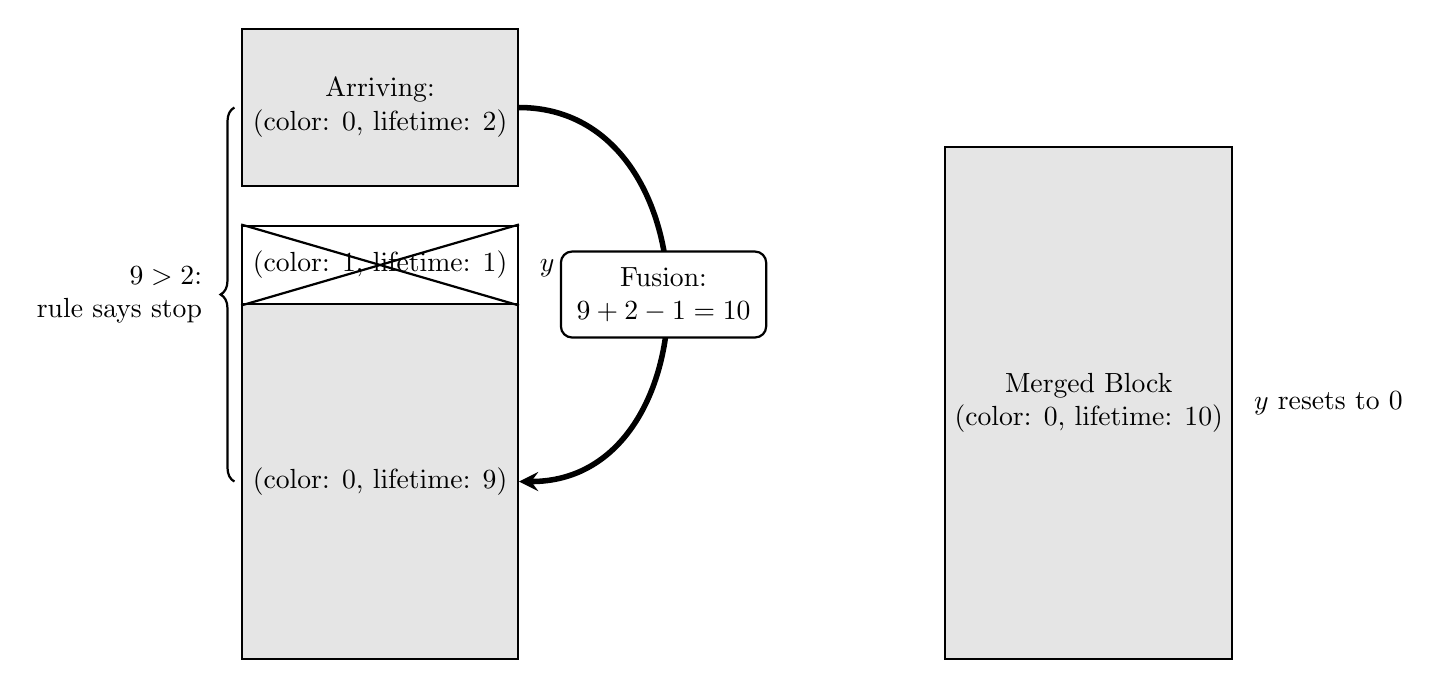
\begin{tikzpicture}[
    block/.style={draw, thick, minimum width=3.5cm, align=center},
    bubble/.style={draw, thick, rounded corners, align=center, fill=white, inner sep=2mm},
    >=stealth
]

\gid{bottom-block}{
    \node[block, minimum height=4.5cm, fill=black!10] (bottom) at (0, 2.25) {(color: 0, lifetime: 9)};
}

\gid{red-block}{
    \node[block, minimum height=1cm, fill=white] (red) at (0, 5) {(color: 1, lifetime: 1)};
}

\gid{new-block}{
    \node[block, minimum height=2cm, fill=black!10] (new) at (0, 7) {Arriving:\\(color: 0, lifetime: 2)};
}

\gid{size-check-note}{
    \draw[decorate, decoration={brace, amplitude=5pt}, thick] (-1.85, 2.25) -- (-1.85, 7) node[midway, left=8pt, align=right] {$9 > 2$: \\ rule says stop};
}

\gid{red-block-crossout}{
    \draw[thick] (red.south west) -- (red.north east);
    \draw[thick] (red.north west) -- (red.south east);
}

\gid{obstacle-label}{
    \node[right=4pt] at (red.east) {$y = 1$};
}

\gid{merge-arrow}{
    \draw[->, line width=2pt] (new.east) .. controls +(0:2.5) and +(0:2.5) .. (bottom.east);
}

\gid{fusion-formula}{
    \node[bubble] at (3.6, 4.625) {Fusion:\\$9 + 2 - 1 = 10$};
}

\gid{merged-block}{
    \node[block, minimum height=6.5cm, fill=black!10] (merged) at (9, 3.25) {Merged Block\\(color: 0, lifetime: 10)};
}

\gid{reset-label}{
    \node[right=4pt, align=left] at (merged.east) {$y$ resets to $0$};
}

\end{tikzpicture}